\documentclass[10pt]{article}
\usepackage{graphicx}
\usepackage[none]{hyphenat}
\usepackage{listings}
\usepackage[english]{babel}
\usepackage{siunitx}
\usepackage{caption}
\usepackage{booktabs}
\usepackage{array}
\usepackage{extarrows}
\usepackage{enumerate}
\usepackage{enumitem}
\usepackage{amsmath}
\usepackage{commath}
\usepackage{gensymb}
\usepackage{amssymb}
\usepackage{multicol}
\usepackage[utf8]{inputenc}
\lstset{
 frame=single,
 breaklines=true
}
\usepackage{hyperref}
%\usepackage[margin=0.8in]{geometry}
%\usepackage{exsheets}% also loads the `tasks' package
\usepackage{atbegshi}

%new macro definitions
\renewcommand{\labelenumi}{(\alph{enumi})}
\newcommand{\mydet}[1]{\ensuremath{\begin{vmatrix}#1\end{vmatrix}}}
\providecommand{\brak}[1]{\ensuremath{\left(#1\right)}}
\newcommand{\solution}{\noindent \textbf{Solution: }}
\newcommand{\myvec}[1]{\ensuremath{\begin{pmatrix}#1\end{pmatrix}}}
\newenvironment{amatrix}[1]{%
 \left(\begin{array}{@{}*{#1}{c}|c@{}}
}{%
 \end{array}\right)
}

\newcommand{\myaugvec}[2]{\ensuremath{\begin{amatrix}{#1}#2\end{amatrix}}}

\let\vec\mathbf{}

\begin{document}
\begin{center}
        \textbf\large{CHAPTER-9 \\ TRIANGLES}
\end{center}
\section{Exercise 11.2}
Question(4).Construct a triangle $XYZ$ in which $\angle{Y}=30\degree$,$\angle{Z}=90\degree$ and $XY+YZ+ZX=11cm$. \\
\textbf{Solution:}\\
Let $\vec{X}$,$\vec{Y}$ and $\vec{Z}$ are the vertices of the triangle with coordinates.
Given $XY+YZ+ZX=8cm$.So the coordinate of the vertice  $\vec{X}$ is:
\begin{align}
{
\vec{X} =\myvec{0\\0}
}
\end{align}
Also given $\angle{Y}=30\degree$ and $\angle{Z}=90\degree$ so by finding the length of sides we can form a required triangle. \\
 The input parameters for this construction are\\
 \begin{table}[h]
	 \centering
	  \begin{tabular}{|c|c|c|} 
  \hline 
  \textbf{Symbol}&\textbf{Value}&\textbf{Description}\\ 
  \hline 
  $c+a+b$ & 11 & $XY+YZ+ZX$ \\ 
  \hline 
 $\angle{Y}$ & 30$\degree{}$ & $\angle{Y}$ in $\triangle$$ABC$\\ 
  \hline 
        $\angle{Z}$ & 90$\degree{}$ & $\angle{Z}$ in $\triangle$$XYZ$ \\
   
  \hline  
 $\vec{e_1}$ & $\myvec{ 
   1 \\
   0 \\
   0 
   }$ & Basis vector\\ 
 \hline
 \end{tabular}\\	

	 \caption{Parameters}
	 \label{tab:table1}
 \end{table}\\
From the given information\\
 \begin{align}
     a+b+c=k\\
	 b\cos{Z}+c\cos{Y}-a=0\\
	 b\sin{Z}-c\sin{Y}=0
 \end{align}
 Resulting in the matrix equations:
 \begin{align}
	 \myvec{1 & 1 & 1\\-1 & \cos{Z} & \cos{Y}\\0 & \sin{Z} & -\sin{Y}}\myvec{a \\ b \\ c}=k\vec{e_1}
 \end{align}
 Substituting the values of $k$,$\vec{e_1}$,$\angle{Y}$,$\angle{Z}$
 \begin{align}
     \myvec{1 & 1 & 1\\-1 & \cos{90\degree} & \cos{30\degree}\\ 0 & \sin{90\degree} & -\sin{30\degree}}\myvec{a \\ b \\ c}= 11\myvec{1 \\ 0 \\ 0 }
 \end{align}
  \begin{align}
	  \myvec{1 & 1 & 1\\-1 & 0 & \sqrt{3}/2\\0 &  1 & -1/2}\myvec{a \\ b \\c}= \myvec{11 \\ 0 \\ 0 }
  \end{align}
 Using row reduction methods to bring the values of $a$,$b$,$c$ into row-reduced echelon form using augumented matrix,

\begin{align}
     \myaugvec{3}{1 & 1 & 1 & 11\\ 0 & 1 & \frac{\sqrt{3}}{2}+1 & 0\\0 &  1 & \frac{-1}{2} & 0} \\
     \xleftrightarrow[]{R_2 \rightarrow R_2+R_1}\myaugvec{3}{1 & 1 & 1 & 11\\ 0 & 1 & \frac{\sqrt{3}}{2}+1 & 11\\ 0 &  1 & \frac{-1}{2} & 0}\\
    \xleftrightarrow[]{R_1 \rightarrow R_1-R_2}\myaugvec{3}{1 & 0 & \frac{-\sqrt{3}}{2} & 0\\0 & 1 & \frac{\sqrt{3}}{2}+1 & 11\\0 &  0 & \frac{-1}{2} & 0}\\
    \xleftrightarrow[]{R_3 \rightarrow R_3-R_2}\myaugvec{3}{1 & 0 & \frac{-\sqrt{3}}{2} & 0\\0 & 1 & \frac{\sqrt{3}}{2}+1 & 11\\0 &  0 & \frac{-\sqrt{3}-3}{2} & -11}\\
    \xleftrightarrow[]{R_3 \rightarrow \frac{2}{-\sqrt{3}-3} R_3}\myaugvec{3}{1 & 0 & \frac{-\sqrt{3}}{2} & 0\\0 & 1 & \frac{\sqrt{3}}{2}+1 & 11 \\0 &  0 & 1 & \frac{22}{3+\sqrt{3}}}\\
    \xleftrightarrow[]{R_1 \rightarrow R_1+\frac{\sqrt{3}}{2}R_2}\myaugvec{3}{1 & 0 & 0 & \frac{11\sqrt{3}}{3+\sqrt{3}} \\ 0 & 1 & \frac{\sqrt{3}}{2}+1 & 11\\0 &  0 & 1 & \frac{22}{3+\sqrt{3}} }\\
    \xleftrightarrow[]{R_2 \rightarrow R_2-\frac{(\sqrt{3}}{2}+1)R_3}\myaugvec{3}{1 & 0 & 0 & \frac{11\sqrt{3}}{3+\sqrt{3}} \\ 0 & 1 & 0 & 11(1-\frac{\sqrt{3}+2}{\sqrt{3}+3})\\0 &  0 & 1 & \frac{22}{3+\sqrt{3}}}
 \end{align} 

 After reduction the values of $a$,$b$,$c$ are:
 \begin{align}
     \myvec{a \\ b \\ c}=\myvec{\frac{11\sqrt{3}}{3+\sqrt{3}} \\ 11(1-\frac{\sqrt{3}+2}{\sqrt{3}+3}) \\\frac{22}{3+\sqrt{3}}}
 \end{align}
 Therefore the coordinates of the vertices are:
 \begin{align}
      \vec{X}=\myvec{0\\0}\\
      \vec{Z}=\myvec{b \\ 0}=\myvec{11(1-\frac{\sqrt{3}+2}{\sqrt{3}+3}) \\ 0}\\                                               
      \vec{Y}=\myvec{b \\ a}=\myvec{11(1-\frac{\sqrt{3}+2}{\sqrt{3}+3}) \\ \frac{11\sqrt{3}}{3+\sqrt{3}} }
 \end{align}
 Construction:\\
 \begin{figure}[h]
	 \begin{center}
		 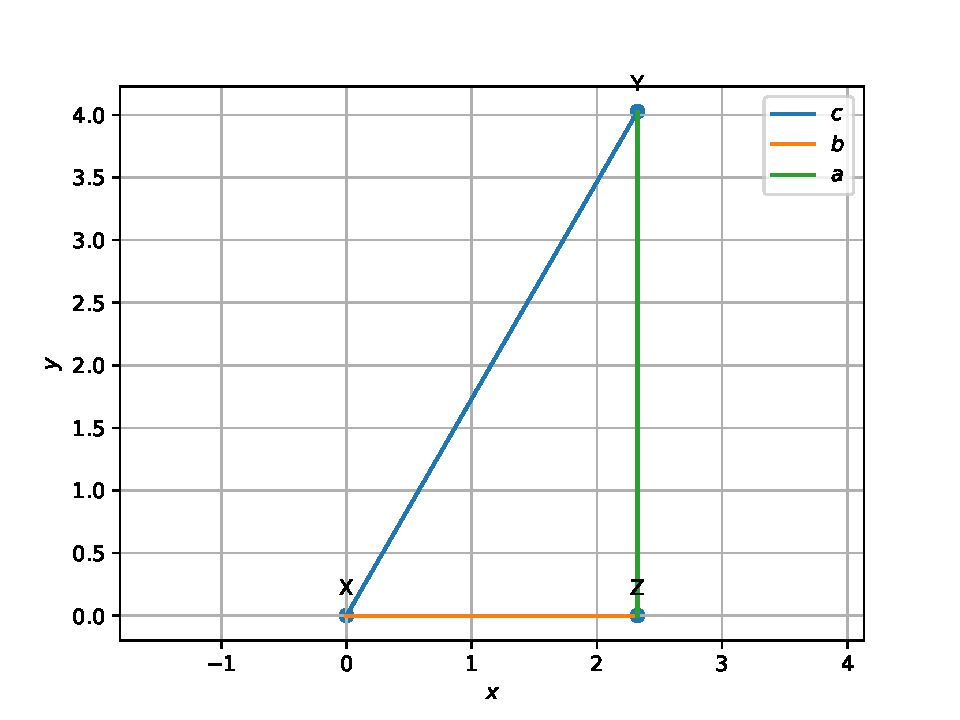
\includegraphics[width=\columnwidth]{code(m)/fig.pdf}
	 \end{center}
	 \caption{Triangle XYZ}
	 \label{fig:Fig1}
 \end{figure}

\end{document}
